\section{Our Work}
(1) To design and implement deep learning based attack detection mechanism.

(2) This work has used self taught deep learning scheme in which unsupervised feature learning has been employed on training data.

(3) The learnt features were applied to the labeled test dataset for classification into attack and normal.
\section{Dataset description}
We used NSL-KDD intrusion dataset which is available in csv format for
model validation and evaluations.
The original dataset consists of 125,973 records of train and 22,544 records of test, each with 41 features such as duration,protocol, service, flag, source bytes, destination bytes, etc.

\begin{figure}[h]
	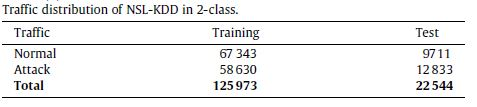
\includegraphics[width=\linewidth]{Capture17.JPG}
	\caption{}
	\label{fig:boat1}
\end{figure}
\newpage
\begin{figure}[t]
	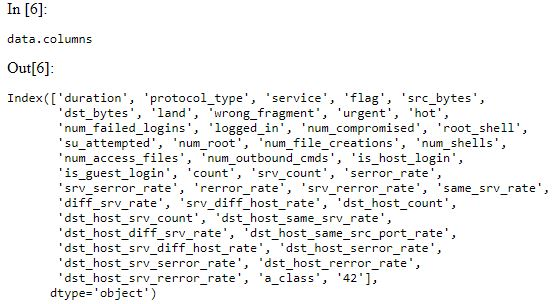
\includegraphics[width=\linewidth]{Capture10.JPG}
	\caption{columns of dataset}
	\label{}
\end{figure}
\begin{figure}[h]
	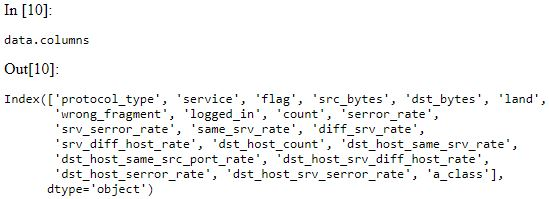
\includegraphics[width=\linewidth]{Capture11.JPG}
	\caption{columns of dataset after droping some columns}
	\label{}
\end{figure}

\section{Our Approach}
\textbf{ToolS/Framework Used -}  Anaconda, Spider IDE, Keras, Sklearn .

\textbf{Anaconda} is complete development environment with over 300 Python packages.Conda is a powerful package manager and environment manager that you use with command line commands at the Anaconda Prompt.

\textbf{Keras} is a high-level neural networks API, written in Python and capable of running on top of TensorFlow, CNTK, or Theano.

The core data structure of Keras is a model, a way to organize layers. The simplest type of model is the Sequential model, a linear stack of layers. For more complex architectures, you should use the Keras functional API, which allows to build arbitrary graphs of layers.

Before training the network, categorical features have been encoded into discrete features using 1-to-n encoding technique.
\newline
\textbf{Labelencoder()} is a utility function to help normalize labels such that they contain only values between 0 and n\_classes-1.

\textbf{fit\_transform()} joins two steps and first step is  initial fitting of parameters on the training set,in second step it returns a transformed set. Internally, it just calls first fit() and then transform()on the same data.

\textbf{MinMaxScaler} Transforms features by scaling each feature to a given range.
This translates each feature individually such that it is in the given range on the training set, i.e. between zero and one.

\textbf{k-Fold Cross Validation} 
\newline
The main standard for machine learning model evaluation is k-fold cross validation.
It provides a estimate of the performance of a model on unseen data. It does this by splitting the training dataset into k subsets and takes turns training models on all subsets except one which is held out, and evaluating model performance on the held out validation dataset. The process is repeated until all subsets are given an opportunity to be the held out validation set. The performance measure is then averaged across all models that are created.
Cross validation is often not used for evaluating deep learning models because of the greater computational expense. For example k-fold cross validation is often used with 5 or 10 folds. As such, 5 or 10 models must be constructed and evaluated, greatly adding to the evaluation time of a model.
Nevertheless, it when the problem is small enough or if you have sufficient compute resources, k-fold cross validation can give you a less biased estimate of the performance of your model.
In our approach we used the handy StratifiedKFold class from the sk-learn Python machine learning library to split up the training dataset into 10 folds. The folds are stratified, meaning that the algorithm attempts to balance the number of instances of each class in each fold.

\newpage
\begin{figure}[h]
	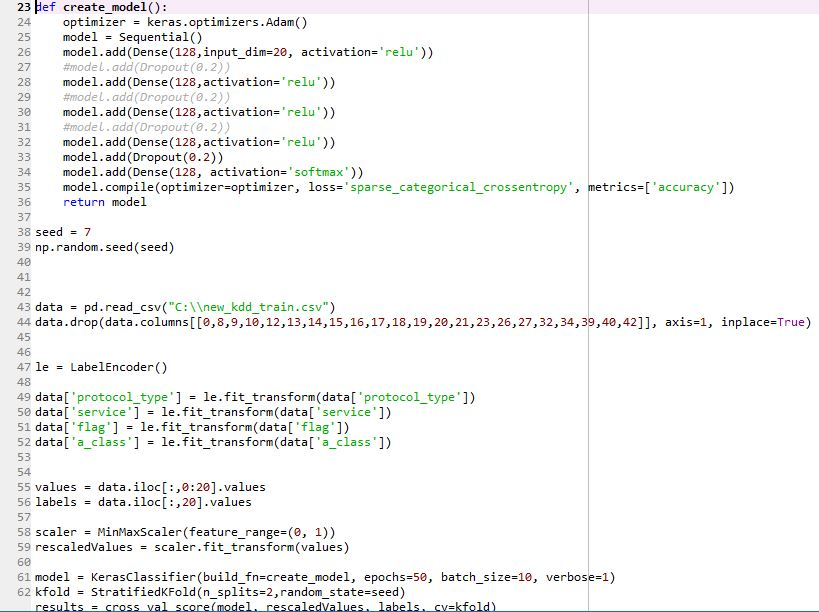
\includegraphics[width=\linewidth]{Capture19.JPG}
	\caption{}
	\label{fig:boat1}
\end{figure}

\newpage
\section{Accuracy of our model :}
\begin{figure}[h]
	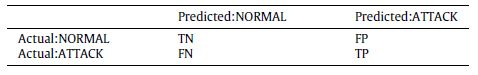
\includegraphics[width=\linewidth]{Capture14.JPG}
	\caption{}
	\label{fig:boat1}
\end{figure}
\begin{figure}[h]
	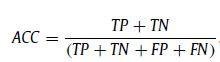
\includegraphics[width=\linewidth]{Capture15.JPG}
	\caption{Accuracy Formula}
	\label{fig:boat1}
\end{figure}
\begin{figure}[h]
	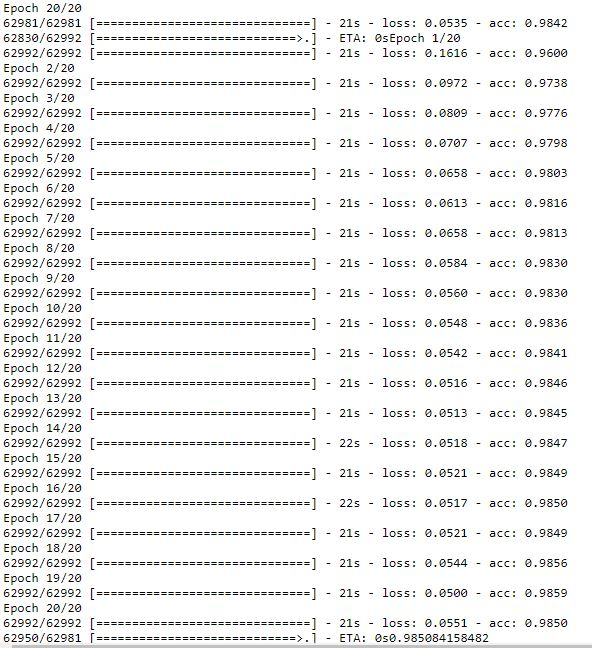
\includegraphics[width=\linewidth]{Capture12.JPG}
	\caption{Accuracy}
	\label{fig:boat1}
\end{figure}



